% arara: xelatex
% arara: xelatex
% arara: xelatex

% options:
% thesis=B bachelor's thesis
% thesis=M master's thesis
% czech thesis in Czech language
% english thesis in English language
% hidelinks remove colour boxes around hyperlinks

\documentclass[thesis=B,czech]{FITthesis}[2019/03/21]

\usepackage[utf8]{inputenc}

\usepackage{dirtree}

\newcommand{\tg}{\mathop{\mathrm{tg}}} %cesky tangens
\newcommand{\cotg}{\mathop{\mathrm{cotg}}} %cesky cotangens

% % % % % % % % % % % % % % % % % % % % % % % % % % % % % % 
% ODTUD DAL VSE ZMENTE
% % % % % % % % % % % % % % % % % % % % % % % % % % % % % % 

\department{Katedra teoretické informatiky}
\title{Příklad vyplněné šablony}
\authorGN{Jan} %(křestní) jméno (jména) autora
\authorFN{Nový} %příjmení autora
\authorWithDegrees{Jan Nový} %jméno autora včetně akademických titulů
\author{Jan Nový} %jméno autora bez akademických titulů
\supervisor{doc. Ing. Marek Navrátil}
\acknowledgements{Děkuji všem a za vše. Nevíte-li, co sem napsat, příkaz odstraňte.}
\abstractCS{V~několika větách shrňte obsah a přínos této práce v~češtině. Po přečtení abstraktu by měl mít čtenář dost informací pro rozhodnutí, zda chce Vaši práci číst.}
\abstractEN{Sem doplňte ekvivalent abstraktu Vaší práce v~angličtině.}
\placeForDeclarationOfAuthenticity{V~Praze}
\declarationOfAuthenticityOption{4} %volba Prohlášení
\keywordsCS{Závěrečná práce, \LaTeX{}.}
\keywordsEN{Thesis, \LaTeX{}.}
\website{http://site.example/thesis} %volitelná URL práce, objeví se v tiráži


\begin{document}

\begin{introduction}
	Doplňte úvod Vaší práce.
\end{introduction}

\chapter{Nějaká kapitola}

Doplňte kapitoly Vaší práce.

\section{Nějaká sekce}

Doplňte vhodný text.

\chapter{Další kapitola}


\begin{conclusion}
	Doplňte závěr.
	
\end{conclusion}

\bibliographystyle{csn690}
\bibliography{mybibliographyfile}

\appendix

\chapter{Seznam použitých zkratek}
% \printglossaries
\begin{description}
	\item[GUI] Graphical user interface
	\item[XML] Extensible markup language
\end{description}


% % % % % % % % % % % % % % % % % % % % % % % % % % % 
% Tuto kapitolu z výsledné práce ODSTRAŇTE.
% % % % % % % % % % % % % % % % % % % % % % % % % % % 

\chapter{Návod k~použití této šablony}

Tento dokument slouží jako základ pro napsání závěrečné práce na Fakultě informačních technologií ČVUT v~Praze.

\section{Výběr základu}

Vyberte si šablonu podle druhu práce (bakalářská, diplomová), jazyka (čeština, angličtina) a kódování (ASCII, \mbox{UTF-8}, \mbox{ISO-8859-2} neboli latin2 a nebo \mbox{Windows-1250}). 

V~české variantě naleznete šablony v~souborech pojmenovaných ve formátu práce\_kódování.tex. Typ práce může být:
\begin{description}
	\item[BP] bakalářská práce,
	\item[DP] diplomová (magisterská) práce.
\end{description}
Kódování zdrojového souboru (\LaTeX{}), ve kterém chcete psát, může být:
\begin{description}
	\item[UTF-8] kódování Unicode,
	\item[ISO-8859-2] latin2,
	\item[Windows-1250] znaková sada 1250 Windows.
\end{description}
V~případě nejistoty ohledně kódování doporučujeme následující postup:
\begin{enumerate}
	\item Otevřete šablony pro kódování UTF-8 v~editoru prostého textu, který chcete pro psaní práce použít -- pokud můžete texty s~diakritikou normálně přečíst, použijte tuto šablonu.
	\item V~opačném případě postupujte dále podle toho, jaký operační systém používáte:
	\begin{itemize}
		\item v~případě Windows použijte šablonu pro kódování \mbox{Windows-1250},
		\item jinak zkuste použít šablonu pro kódování \mbox{ISO-8859-2}.
	\end{itemize}
\end{enumerate}


V~anglické variantě jsou šablony pojmenované podle typu práce, možnosti jsou:
\begin{description}
	\item[bachelors] bakalářská práce,
	\item[masters] diplomová (magisterská) práce.
\end{description}

\section{Použití šablony}

Šablona je určena pro zpracování systémem \LaTeXe{}. (Začátečníci v~\LaTeX{}u mohou využít např. \cite{rybicka}.) Text je možné psát v~textovém editoru jako prostý text, lze však také využít specializovaný editor pro \LaTeX{}, např. Kile.

Pro získání tisknutelného výstupu z~takto vytvořeného souboru použijte příkaz \verb|pdflatex|, kterému předáte cestu k~souboru jako parametr. Vhodný editor pro \LaTeX{} toto udělá za Vás. \verb|pdfcslatex| ani \verb|cslatex| \emph{nebudou} s~těmito šablonami fungovat.

\subsection{Typografie}

Při psaní dodržujte typografické konvence zvoleného jazyka. Česky psané \uv{uvozovky} zapisujte použitím příkazu \verb|\uv|, kterému v~parametru předáte text, jenž má být v~uvozovkách. Anglické otevírací uvozovky se v~\LaTeX{}u zadávají jako dva zpětné apostrofy, uzavírací uvozovky jako dva apostrofy. Často chybně uváděný symbol "{} (palce) nemá s~uvozovkami nic společného.

Dále je třeba zabránit zalomení řádky mezi některými slovy, v~češtině např. za jednopísmennými předložkami a spojkami (vyjma \uv{a}) nebo mezi číslicí a měrnou jednotkou. To docílíte vložením pružné nezalomitelné mezery -- znakem \texttt{\textasciitilde}. V~tomto případě to není třeba dělat ručně, lze použít program \verb|vlna|.

Nezapomeňte také na rozlišení \uv{vodorovných čárek}, které je dáno nejen typografickými zvyklostmi, ale i pravidly českého pravopisu. Pro dělení slov (na konci řádku) nebo jejich spojování nebo v~rámci složenin používejte rozdělovník (v~\LaTeX{}u se zapisuje jako \verb|-|), naopak pomlčku (v~\LaTeX{}u zapsanou jako \verb|--|) užívejte pro význam rozmezí nebo rozsahu a nebo jako větnou pomlčku (namísto interpunkce). Zcela jiným znakem je též mínus (ve stejné výšce a stejné délky jako vodorovná čárka znaku plus), v~\LaTeX{}u se zapisuje pouze v~matematickém režimu.

Více o~typografii viz \cite{kobltypo}.

\subsection{Obrázky}

Pro umožnění vkládání obrázků je vhodné použít balíček \verb|graphicx|, samotné vložení se provede příkazem \verb|\includegraphics|. Takto je možné vkládat obrázky ve formátu PDF, PNG a JPEG jestliže používáte pdf\LaTeX{} nebo ve formátu EPS jestliže používáte \LaTeX{}. Doporučujeme preferovat vektorové obrázky před rastrovými (vyjma fotografií).

\subsubsection{Formáty grafiky}

Z~hlediska reprezentace obrazových informací existuje dělení grafických formátů na rastrové a vektorové. Ty první reprezentují obrázek pomocí barev jednotlivých bodů, ty druhé pomocí informací (souřadnice, barva) o~částech obrázků (úsečka, polygon, plocha). Z~toho plyne vhodnost formátů pro určitý obsah: rastrové pro fotografie, vektorové pro snadno popsatelné obrázky (zejména ty, které obsahují text, jasné tvary apod.). Mezi vektorové souborové formáty patří např. PDF, EPS, SVG, WMF; rastrové obrázky lze najít v~souborech typu PNG, JPEG, GIF, TIFF.

Rastrové obrázky neumožňují, na rozdíl od vektorových, zvětšení beze ztráty vizuálně postřehnutelné kvality. Vzhledem k~vlastnostem grafických formátů a nárokům na vzhled (zejména) vytištěné práce důrazně doporučujeme využít vektorovou grafiku pro všechny obrázky znázorňující typický vektorový obsah (např. diagramy) a rastrové využívat pouze pro fotografie. Důsledně se pro vektorový obsah vyvarujte vkládání grafiky využívající ztrátovou kompresi (JPEG)! Vkládáte-li už do práce rastrovou grafiku, dbejte na dostatečné rozlišení (300 dpi je naprosté minimum). Z~tohoto důvodu je většina obrázků získaných z~webu nevhodná.

\subsubsection{Získání vhodného formátu}

Pro získání vektorových formátů PDF nebo EPS z~jiných lze použít některý z~vektorových grafických editorů. Pro převod rastrového obrázku na vektorový lze použít rasterizaci, kterou mnohé editory zvládají (např. Inkscape). Pro konverze lze použít též nástroje pro dávkové zpracování běžně dodávané s~\LaTeX{}em, např. \verb|epstopdf|. Běžný formát SVG (specifikace viz \cite{svgspec}) sice není možné vkládat přímo (zatím), konverzi však zvládne řada vektorových grafických editorů.

\subsubsection{Plovoucí prostředí}

Příkazem \verb|\includegraphics| lze obrázky vkládat přímo, doporučujeme však použít plovoucí prostředí, konkrétně \verb|figure|. Například obrázek \ref{fig:float} byl vložen tímto způsobem. Vůbec přitom nevadí, když je obrázek umístěn jinde, než bylo původně zamýšleno -- je tomu tak hlavně kvůli dodržení typografických konvencí. Namísto vynucování konkrétní pozice obrázku doporučujeme používat odkazování z~textu (dvojice příkazů \verb|\label| a \verb|\ref|).

\begin{figure}\centering
	
\includegraphics[width=0.5\textwidth, angle=30]{cvut-logo-bw}
	\caption[Příklad obrázku]{Ukázkový obrázek v~plovoucím prostředí}\label{fig:float}
\end{figure}

\subsubsection{Verze obrázků}

% Gnuplot BW i barevně
Může se hodit mít více verzí stejného obrázku, např. pro barevný či černobílý tisk a nebo pro prezentaci. S~pomocí některých nástrojů na generování grafiky je to snadné.

Máte-li například graf vytvořený v~programu Gnuplot, můžete jeho černobílou variantu (viz obr. \ref{fig:gnuplot-bw}) vytvořit parametrem \verb|monochrome dashed| příkazu \verb|set term|. Barevnou variantu (viz obr. \ref{fig:gnuplot-col}) vhodnou na prezentace lze vytvořit parametrem \verb|colour solid|.

\begin{figure}\centering
	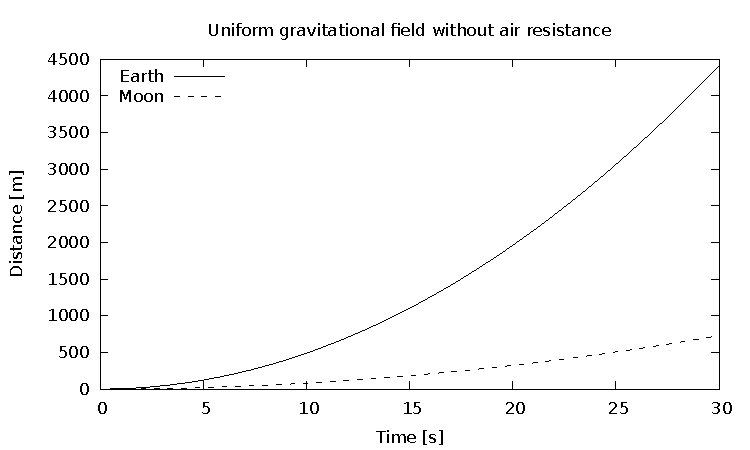
\includegraphics{gnuplot-bw}
	\caption[Gnuplot černobíle]{Černobílá varianta obrázku generovaného programem Gnuplot}\label{fig:gnuplot-bw}
\end{figure}

\begin{figure}\centering
	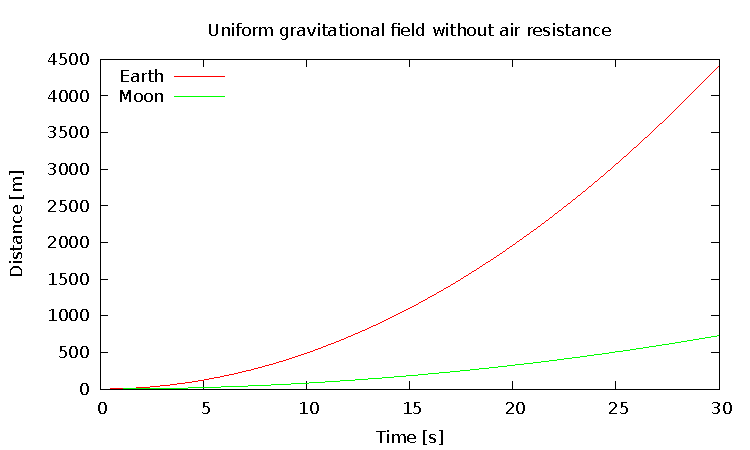
\includegraphics{gnuplot-col}
	\caption[Gnuplot barevně]{Barevná varianta obrázku generovaného programem Gnuplot}\label{fig:gnuplot-col}
\end{figure}


\subsection{Tabulky}

Tabulky lze zadávat různě, např. v~prostředí \verb|tabular|, avšak pro jejich vkládání platí to samé, co pro obrázky -- použijte plovoucí prostředí, v~tomto případě \verb|table|. Například tabulka \ref{tab:matematika} byla vložena tímto způsobem.

\begin{table}\centering
	\caption[Příklad tabulky]{Zadávání matematiky}\label{tab:matematika}
	\begin{tabular}{|l|l|c|c|}\hline
		Typ		& Prostředí		& \LaTeX{}ovská zkratka	& \TeX{}ovská zkratka	\tabularnewline \hline \hline
		Text		& \verb|math|		& \verb|\(...\)|	& \verb|$...$|		\tabularnewline \hline
		Displayed	& \verb|displaymath|	& \verb|\[...\]|	& \verb|$$...$$|	\tabularnewline \hline
	\end{tabular}
\end{table}

\subsection{Literatura}

Vše, čeho nejste autorem (myšlenky, nápady, text, obrázky, \ldots) by mělo být řádně ocitováno -- pokud možno původní zdroj. Vzhledem k~charakteru této práce (odborná) upřednostňujte důvěryhodné a odborné zdroje (existuje-li tištěná verze, citujte raději tu). Důrazně se tedy \emph{vyvarujte citace z~Wikipedie} (kromě odůvodněných a nejnutnějších případů).

Citování (tedy přesné specifikování použitého informačního zdroje a také odkaz na něj z textu) je vhodné provést podobně jako v tomto textu, tedy v souladu s aktuálně platnou normou ČSN ISO 690 \cite{iso690}.

\subsection{Sazba URL}

Pro vkládání URL a podobných informací doporučujeme použít příkaz \verb|url| ze stejnojmenného balíčku. Zajistíte tím jednak odlišení adresy od ostatního textu pomocí jiného písma a také zalamování na konci řádku.

Chcete-li vkládat odkazy (funkční v~PDF), použijte příkaz \verb|href| z~balíčku \verb|hyperref|.

% % % % % % % % % % % % % % % % % % % % % % % % % % % 

\chapter{Obsah přiloženého CD}

Vhodným způsobem vizualizujte obsah přiloženého média. Lze použít balíček \verb|dirtree| a vytvořit např. následující výstup (adresáře src a text s~příslušným obsahem jsou \emph{povinné}):

\begin{figure}
	\dirtree{%
		.1 readme.txt\DTcomment{stručný popis obsahu CD}.
		.1 exe\DTcomment{adresář se spustitelnou formou implementace}.
		.1 src.
		.2 impl\DTcomment{zdrojové kódy implementace}.
		.2 thesis\DTcomment{zdrojová forma práce ve formátu \LaTeX{}}.
		.1 text\DTcomment{text práce}.
		.2 thesis.pdf\DTcomment{text práce ve formátu PDF}.
	}
\end{figure}


\end{document}
